\secnumbersection{PROBLEM DEFINITION} \label{sec:prob}
% ==- CONTEXT -=============================================
\subsection{Context} \label{ssec:prob_context}
% GENERAL DEFINITION OF A PARTICLE ACCELERATOR
A particle accelerator is a machine that can accelerate charged particles to very high speeds and contains them in well-defined beams via an electromagnetic field, providing an environment in which controlled collisions can occur so that particle physicists can study the small particles that result from these impacts~\cite{leduff2005longitudinal}.
It is important to note that due to the fact that the special theory of relativity requires that matter always travels slower than the speed of light in a vacuum, a particle will never reach this speed.
Due to this, the particle's speed is not thought of in traditional terms, but rather in terms of its energy or momentum, usually measured in electron Volts (eV).

As of the time of writing of this work, two types of accelerators are mainly used to study particle physics: the circular or cyclic radiofrequency (RF) and the linear accelerators.
The former is, as the name suggests, a ring, where the particles' track is bent into a circle, allowing them to re-use the same track as much as possible so that they can reach energies up to the order of Tera eV (TeV) in some cases, like the well-known Large Hadron Collider (LHC), at CERN~\cite{leduff2005longitudinal}.
The latter, usually denominated linear particle accelerators (linacs), accelerate particles by attracting them onto charged plates and switching their charge after the particles pass the plate to repel them, pushing them to the next plate.
While the particles accelerated by linacs generally achieve lower momenta than the ones pushed by their circular counterparts, they offer the advantage that they can produce a continuous stream of particles, whereas a cyclic accelerator can only periodically raise the particles to sufficient energy to merit a ``shot'' at the target~\cite{pinchoff2005introduction}.

% BRIEF DESCRIPTION OF JLAB, CEBAF AND CLAS12 (DETECTOR)
At the laboratory for which this work is done, TJNAF or Jefferson Laboratories (JLab) research is assisted by the use of one such linac, the Continuous Electron Beam Accelerator Facility (CEBAF).
CEBAF is composed of a polarized electron source and a pair of superconducting radiofrequency linear accelerators connected to each other by two arc sections that contain steering magnets~\cite{leemann2001continuous}.
The peculiar design of CEBAF allows for the continuous beam characteristic of other linacs, while also being able to reuse the tracks, effectively reaching energies found in an accelerator ten times its size~\cite{leemann2001continuous}.
A picture of CEBAF can be seen in \ref{fig:cebaf}.

    \begin{figure}[ht]
        \centering
        \fbox{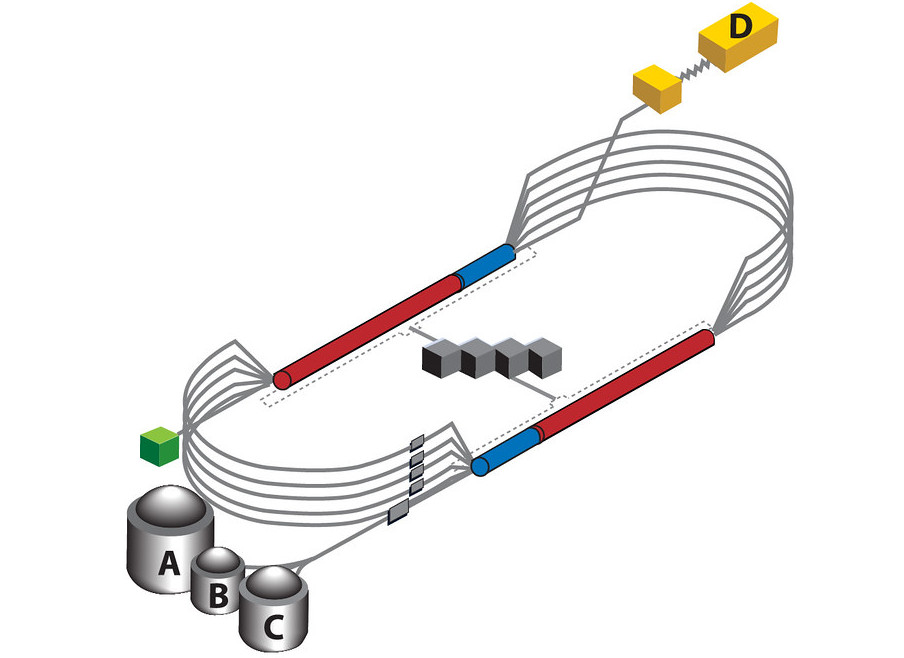
\includegraphics[scale=0.36]{cebaf}}
        \caption{\label{fig:cebaf} The Continuous Electron Beam Accelerator Facility (CEBAF). Source: \texttt{https://www.flickr.com/photos/jeffersonlab/12599705145}}
    \end{figure}

The produced beam ends at one of the four available experimental halls, labeled Hall A, B, C and D, each containing specialized spectrometers to record the products of collisions between the electron beam with itself or with a stationary target.
Particularly, in experimental Hall B, the detector utilized to study the results of these collisions is the CEBAF Large Accelerator Spectrometer for 12 GeV (CLAS12), where each particle-target collision, commonly denominated ``event'', is captured.
This is done in an order of up to several thousand events per second, and the recorded data is later transferred to a farm of computing processors for teams of physicists to analyze them and look for new kinds of particles or information related to the structure of different particles~\cite{mecking2003cebaf}.

% BRIEF DESCRIPTION OF AN EVENT RECONSTRUCTION SOFTWARE
Most particle detectors deal with enormous amounts of data, usually too large to be analyzed ``by hand'' by the physicists trying to understand it, so it's common to build software that aids in the analysis process by filtering the useful data from the background noise~\cite{demchenko2013addressing}.
In the case of CLAS12, this software follows a Service Oriented Architecture (SOA) and consists of the framework, event reconstruction, visualization, calibration, monitoring services as well as detector and event simulator.
The scope of this work is centered mostly with the framework and the event reconstruction software, which are the CLAs12 Reconstruction and Analysis framework (CLARA) and the event reconstruction software itself, specifically with its components associated to the Drift Chambers (DC).

Roughly speaking, the CLARA framework acts as a fairly simple to use system to separate different sections of the software into services which run in so-called Data Processing Environments (DPEs).
The DPEs allow for easy scaling of the software by leaving the distribution of the hardware resources to CLARA~\cite{gyurjyan2013clara,gyurjyan2015component} using the ZeroMQ message transfer protocol~\cite{hintjens2013zeromq}.
The event reconstruction software works by analyzing the data obtained from each of the different components of the CLAS12 detector and tries to reconstruct the event, as its name suggests~\cite{ziegler2013clas12}.

% BRIEF DESCRIPTION OF THE DRIFT CHAMBERS AND THEIR SOFTWARE IMPLEMENTATION
Like any particle detector, CLAS12 is divided into a series of many different components that detect different types of particles utilizing a variety of detection methods~\cite{pinchoff2005introduction}.
One such kind of detectors are the Drift Chambers (DC), which work by measuring the fluctuations in the charge of the matter inside the chambers and in turn try to ``guess'' what passing particle caused such difference in charge.
This measurement is obtained via a set of wires acting as cathodes which, in the case of CLAS12, are strung inside 18 wire chambers inside 3 hexagonal shapes, each with 2 superlayers of 6 layers with 112 wires each, thus having a total of 24,192 wires~\cite{mestayer2017clas}.
These measurements are obtained with the hope that a set or cluster of hits in different wires will allow to estimate the trajectory of the particle that caused these hits and in turn understand its properties.
A diagram of the CLAS12 detector can be seen in Figure \ref{fig:dc_horizontal_cut}, where two particle trajectories are marked in a pointed line.
The wires hit by each trajectory are marked in red in the image to the left and the area that is detected by each wire is denoted by the hexagons in the image to the right.

    \begin{figure}[ht]
        \centering
        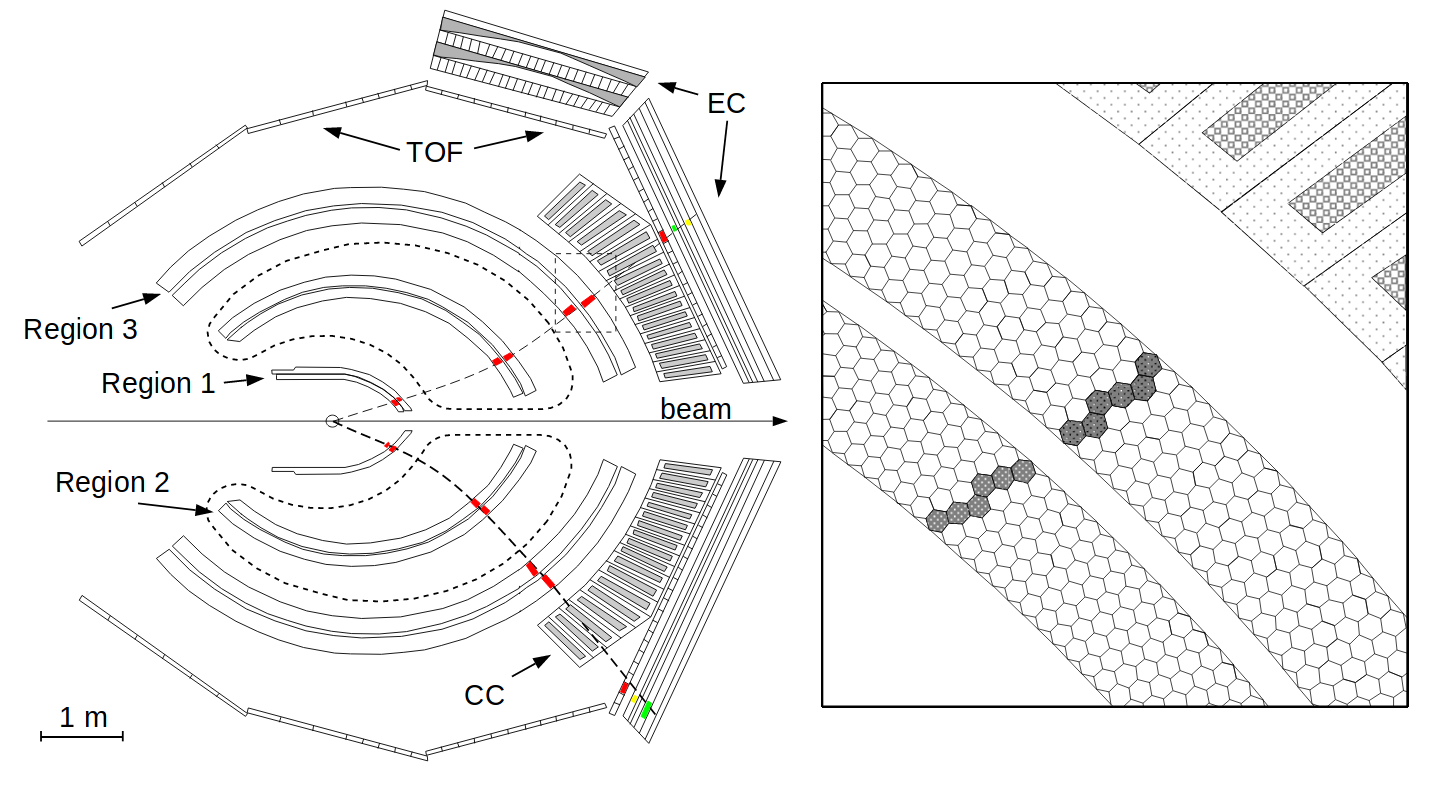
\includegraphics[scale=0.30]{dc/horizontal_cut}
        \caption{\label{fig:dc_horizontal_cut} Horizontal cut through the CLAS detector at beam line elevation showing two charged particles traversing the $18$ superlayers in the $3$ regions of the drift chambers in opposite sectors. The picture to the right shows an enlargement of the boxed area in the picture to the left. Source: The CLAS Drift Chamber System~\cite{mestayer2000clas}.}
    \end{figure}

% ==- THE PROBLEM -=========================================
\subsection{The Problem} \label{ssec:prob_the_problem}
% BRIEF DESCRIPTION OF PARTICLE TRACKING AND THE KALMAN FILTER
Different algorithms are used to estimate the trajectory or track of some of the particles that are ejected in each event, and these algorithms belong in a field named particle tracking.
In the specific case of the DC in CLAS12, particle tracking is done via the Extended Kalman Filter (EKF), which is a popular algorithm for estimating the position of a moving object with a good precision given that the path followed by it can be modeled by deterministic movement equations and that measurements (i.e: the ones taken by the wires) can be obtained for this object's position over time.
This makes it a good estimator for the charged particles ejected by the target after each event~\cite{kalman1960new}.

The EKF shows great performance at its task in the reconstruction software, but it suffers from the disadvantage that it is a fairly slow algorithm.
To reach the previously mentioned precision, both the Kalman Filter (KF) and its extended counterpart require matrix multiplications and inversions when computing states, as well as the calculation of Jacobian matrices, as is described in Section \ref{ssec:framework_ekf}.
These matrix operations mean that the computational complexity of the algorithm is quite high, which in big-O notation is:
    \begin{equation*}
        O(\text{C}(\mathbf{f}(\cdot, \cdot)) + \text{C}(\mathbf{h}(\cdot)) + n^3 + n^2\,m + n\,m^2)\,,
    \end{equation*}

% \newpage

where $n$ and $m$ are the state and measurement vector sizes and $C(\mathbf{f}(\cdot, \cdot))$ along with $C(\mathbf{h}(\cdot))$ are used to denote the costs of $\mathbf{f}(\cdot, \cdot)$ and $\mathbf{h}(\cdot)$ respectively, where $\mathbf{f}$ and $\mathbf{h}$ are the transition functions between two arbitrary timesteps $k$ and $k+1$ for the state vector $\mathbf{x}_k$ and the measurement vector $\mathbf{z}_k$ respectively.
The mathematical formulation of the model and the calculation of the computational complexity of each operation are described in detail in Section \ref{ssec:framework_ekf}.

Something to note is that while most systems using the Kalman Filter are slowed down because they process large state and measurement vectors with large covariance matrices, the DC software suffers from a different issue.
The $n$ and $m$ mentioned before are constants $5$ and $6$ respectively, but the state transition itself between states $k$ and $k+1$ takes a large amount of time and is iterated over a large number of times as is described in Sections \ref{ssec:framework_ekf}, \ref{ssec:framework_tf} and \ref{ssec:framework_rk4}.
Even more, the Kalman Filter is used as a fixed point iteration to compute the state vector at the last measurement site $K$ with enough precision, requiring many runs to obtain precise results.

This large computation time takes a heavy toll on the total running time of the two engines that process the DC data in the reconstruction software: the DC Hit-Based tracking engine (DCHB) and the DC Time-Based tracking engine (DCTB); taking a total of $49.3\%$ of the total running time of the whole CLAS12 software.
It's also worth noting that the second component in terms of processing time is the Cluster Finding used in DCHB and DCTB, which takes in total a $40.1\%$ of the previously mentioned time.
To better visualize the impact on the processing time of the DCHB and DCTB components, see Figure \ref{fig:engines-times-sep2018}.
As all the other performance tests in this document, these measurements were obtained by running the CLAS12 software on $10.000$ events with real experimental data.
The test file used is named \texttt{clas\_004013.0.hipo}, and can be obtained by contacting the Hall B team at Jefferson Lab (https://www.jlab.org/Hall-B/).

    \begin{figure}[ht] % Note: Maybe I could mention the github's HEAD used to obtain this?
        \centering
        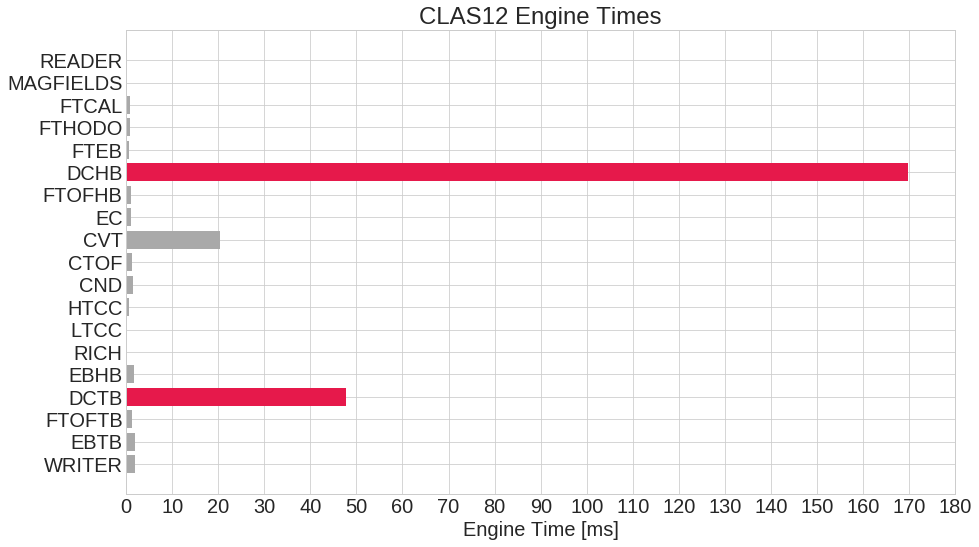
\includegraphics[scale=0.44]{engine_times/1_0}
        \caption{\label{fig:engines-times-sep2018} CLAS12 Engine times as of September 7th, 2018.}
    \end{figure}

The problem that this project focuses on is that of reducing the total computation time of the whole CLAS12 offline software.
To tackle the problem, the project focuses in the slowest components of CLAS12, DCHB and DCTB, and especifically to the acceleration of the Kalman Filter used in these two DC engines.
Another smaller part of the project also focuses in the acceleration of the cluster finding algorithm, considering that it is the second largest bottleneck in the software's execution.

% \newpage

% ==- GOALS -=============================================== %
\subsection{Goals} \label{ssec:prob_goals}
As can be seen in Figure \ref{fig:engines-times-sep2018}, the combined time taken by the DCHB and DCTB engines is as much as $86.35$\% of the total execution time of the CLAS12 software, making them prime candidates for accelerating the reconstruction software.
Therefore, the main goal of this project is to reduce the total running time of the CLAS12 software by specifically accelerating the KF algorithm currently implemented in the code while also trying to tackle the cluster finding algorithm to a lesser extent.
The project's major goals are:

\newpage

    \begin{itemize}
        \item Compare a set of the different Java profilers and analyze which one is the most useful to measure the CLAS12 software performance.
        \item Study which components of the KF and Cluster Finding algorithms implemented in CLAS12 can be accelerated via optimizations and/or parallelization.
        \item Study the way in which these optimizations and/or parallelizations could take place in the context of execution of the software, the CLARA framework.
        \item Effectively apply the optimizations and implement the algorithms that would allow a substantial improvement in the running time of the software.
        \item Profile and test the code continuously while applying changes, ensuring that the output data is consistently the same through the development process.
        \item Document the changes made to the code and describe in detail the algorithms and optimizations implemented in order to help future related work.
    \end{itemize}

It's worth noting that these objectives differ slightly from the ones originally proposed for this project: Originally only parallelization techniques were going to be tested, but during development it was decided to apply general optimizations.